\documentclass[11pt]{article}
\usepackage[margin=1in]{geometry}
\usepackage{graphicx}
\usepackage{amsmath}
\usepackage{booktabs}
\title{A Finite Intercept Correction Calculation}
\author{Anonymous}
\date{}

\begin{document}
\maketitle

\begin{abstract}
This teaching note connects residual averaging to least-squares intercept fitting through five synthetic observations. With the baseline predictor fixed at $2x$ and targets satisfying $y_i=2x_i+3$, every baseline residual equals $3$. Their mean gives the fitted offset $b=3$. A sum-of-squares decomposition explains both this choice and the resulting exact agreement. Mean absolute and mean squared errors at three supplied offsets are algebraically determined and reproduced by a deterministic R calculation. A table and two figures support instruction in residual centering, error aggregation, and the interpretation of errors on observations used for fitting.
\end{abstract}

\section{Introduction}

The intended audience is students beginning regression who understand sample means and squared errors. The educational objective is to connect three operations often introduced separately: computing residuals, fitting an intercept, and summarizing errors. Readers should be able to derive the fitted offset, explain why zero error occurs in this construction, and identify which observations determine each reported quantity.

The example fixes the baseline $f_0(x)=2x$ and supplies
\[
x=(-2,-1,0,1,2), \qquad y=(-1,1,3,5,7).
\]
Only an additive scalar $b$ is fitted. Holding the baseline fixed isolates the role of the intercept: its estimation shifts every prediction by the same amount while preserving the supplied slope. The derivation, computational flow, and error table provide complementary ways to inspect this elementary calculation.

\section{Related Work}

Residual examination supports numerical and graphical understanding of fitted models \cite{Anscombe1963ExaminationAnalysis}. Here, residuals provide the quantities from which the offset is computed. Gneiting \cite{Gneiting2011MakingEvaluating} discusses matching error scores to evaluation objectives; this note makes the absolute and squared aggregations explicit. Efron \cite{Efron1986HowBiased} distinguishes apparent error, calculated using fitting observations, from prediction error on future observations. That distinction determines how to interpret the table below: its entries describe agreement on the same five observations that determine the offset.

\section{Method}

\subsection{Finite Calculation and Error Definitions}

For $i=1,\ldots,5$, define the baseline predictions and residuals by
\[
\hat y_i^{(0)}=2x_i,\qquad r_i=y_i-\hat y_i^{(0)}.
\]
The supplied values give
\[
\hat y^{(0)}=(-4,-2,0,2,4),\qquad r=(3,3,3,3,3).
\]
An offset produces $\hat y_i(b)=2x_i+b$ and residual
$e_i(b)=r_i-b$. The error summaries are
\[
\operatorname{MAE}(b)=\frac{1}{5}\sum_{i=1}^{5}|r_i-b|,
\qquad
\operatorname{MSE}(b)=\frac{1}{5}\sum_{i=1}^{5}(r_i-b)^2.
\]
Thus the data construction directly implies
\[
\operatorname{MAE}(b)=|3-b|,
\qquad
\operatorname{MSE}(b)=(3-b)^2.
\]
The tabulated values are evaluations of these identities at the three supplied settings.

\subsection{Mean Residual Correction and Computational Flow}

Fitting the intercept with the baseline fixed means choosing $b$ to minimize the residual sum of squares. Let
$\bar r=\frac{1}{5}\sum_{i=1}^{5}r_i$. Expanding around this mean gives
\[
\sum_{i=1}^{5}(r_i-b)^2
=
\sum_{i=1}^{5}(r_i-\bar r)^2
+5(b-\bar r)^2.
\]
The cross term vanishes because $\sum_i(r_i-\bar r)=0$.
The first term is independent of $b$, and the second is uniquely minimized at
\[
b^\star=\bar r=\frac{3+3+3+3+3}{5}=3.
\]
This establishes the mean-residual correction as the least-squares intercept for the fixed baseline.

Subtracting the mean centers the residuals. In this construction,
$r_i=\bar r$ at every index, so every centered residual is zero and
$\hat y(3)=(-1,1,3,5,7)=y$. The decomposition makes the reason for exact agreement explicit: all baseline discrepancies are the same constant.

Figure~\ref{fig:residual_workflow} supports tracing dependencies. Targets enter both residual computation and error evaluation; the dashed path highlights that reuse. Students can follow the arrows to distinguish the supplied baseline from the fitted offset and the resulting predictions.

\begin{figure}[!htbp]
    \centering
    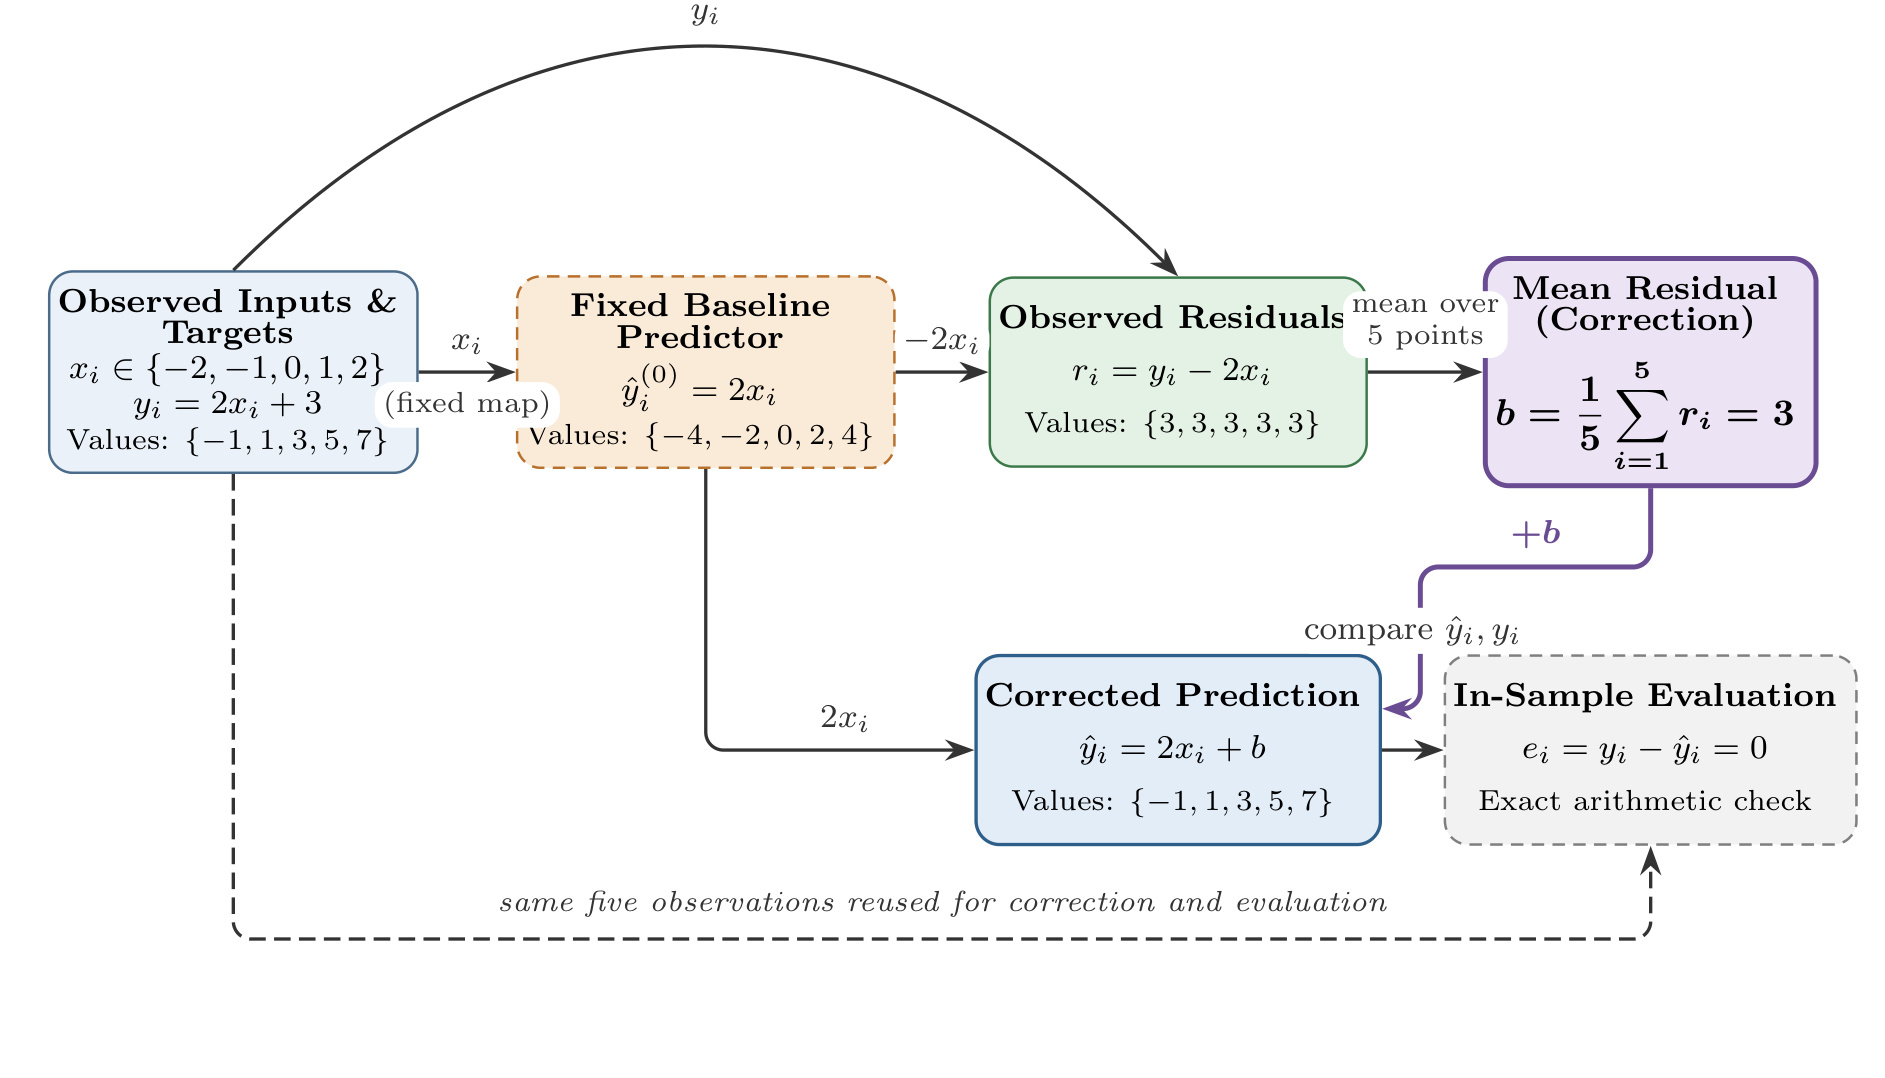
\includegraphics[width=\linewidth]{figures/fig_residual_workflow.jpg}
    \caption{Computational dependencies for the five supplied observations.
    Baseline residuals determine their mean $b=3$, which shifts the fixed
    predictions to the targets. The dashed path identifies the observations
    shared by intercept fitting and in-sample evaluation.}
    \label{fig:residual_workflow}
\end{figure}

\section{Experiments}

\subsection{Observations and Evaluation Protocol}

The supplied experiment is one deterministic base R calculation. It computes the mean of $y-2x$ and evaluates offsets $b=0,1.5,3$ against all five targets. These are three settings within that calculation. Throughout, the baseline slope remains $2$.

The calculation reproduces quantities specified by the algebra. Its results should therefore be read as an arithmetic check and a demonstration of fitting-observation error. The observation set used to calculate each error is exactly the set used to obtain $b^\star$.

\subsection{Computed Errors and Reproducible Figures}

Table~\ref{tab:recorded_errors} reproduces the supplied R results. At $b=0$, each residual is $3$. Adding $1.5$ leaves each residual equal to $1.5$, so MAE becomes $1.5$ and MSE becomes $2.25$. At $b=3$, both summaries are zero.

\begin{table}[!htbp]
    \centering
    \caption{Computed errors from the supplied deterministic R calculation.
    Every entry also follows exactly from
    $\operatorname{MAE}(b)=|3-b|$ and
    $\operatorname{MSE}(b)=(3-b)^2$.}
    \label{tab:recorded_errors}
    \begin{tabular}{rrr}
        \toprule
        Added $b$ & Mean absolute error & Mean squared error \\
        \midrule
        0   & 3   & 9    \\
        1.5 & 1.5 & 2.25 \\
        3   & 0   & 0    \\
        \bottomrule
    \end{tabular}
\end{table}

The intermediate setting illustrates the difference between error aggregations: halving the common residual halves its absolute value and quarters its square. This comparison concerns the arithmetic of the two summaries on these observations.

Figure~\ref{fig:intercept_error} provides a visual reading exercise using exactly the three supplied MSE values. Its source specifies these coordinates directly. The plot and table are two presentations of the same quantities, while the derivation explains them. A useful instructional check is to calculate the intermediate point before reading its annotation and then explain the zero point using the residual decomposition.

\begin{figure}[!htbp]
    \centering
    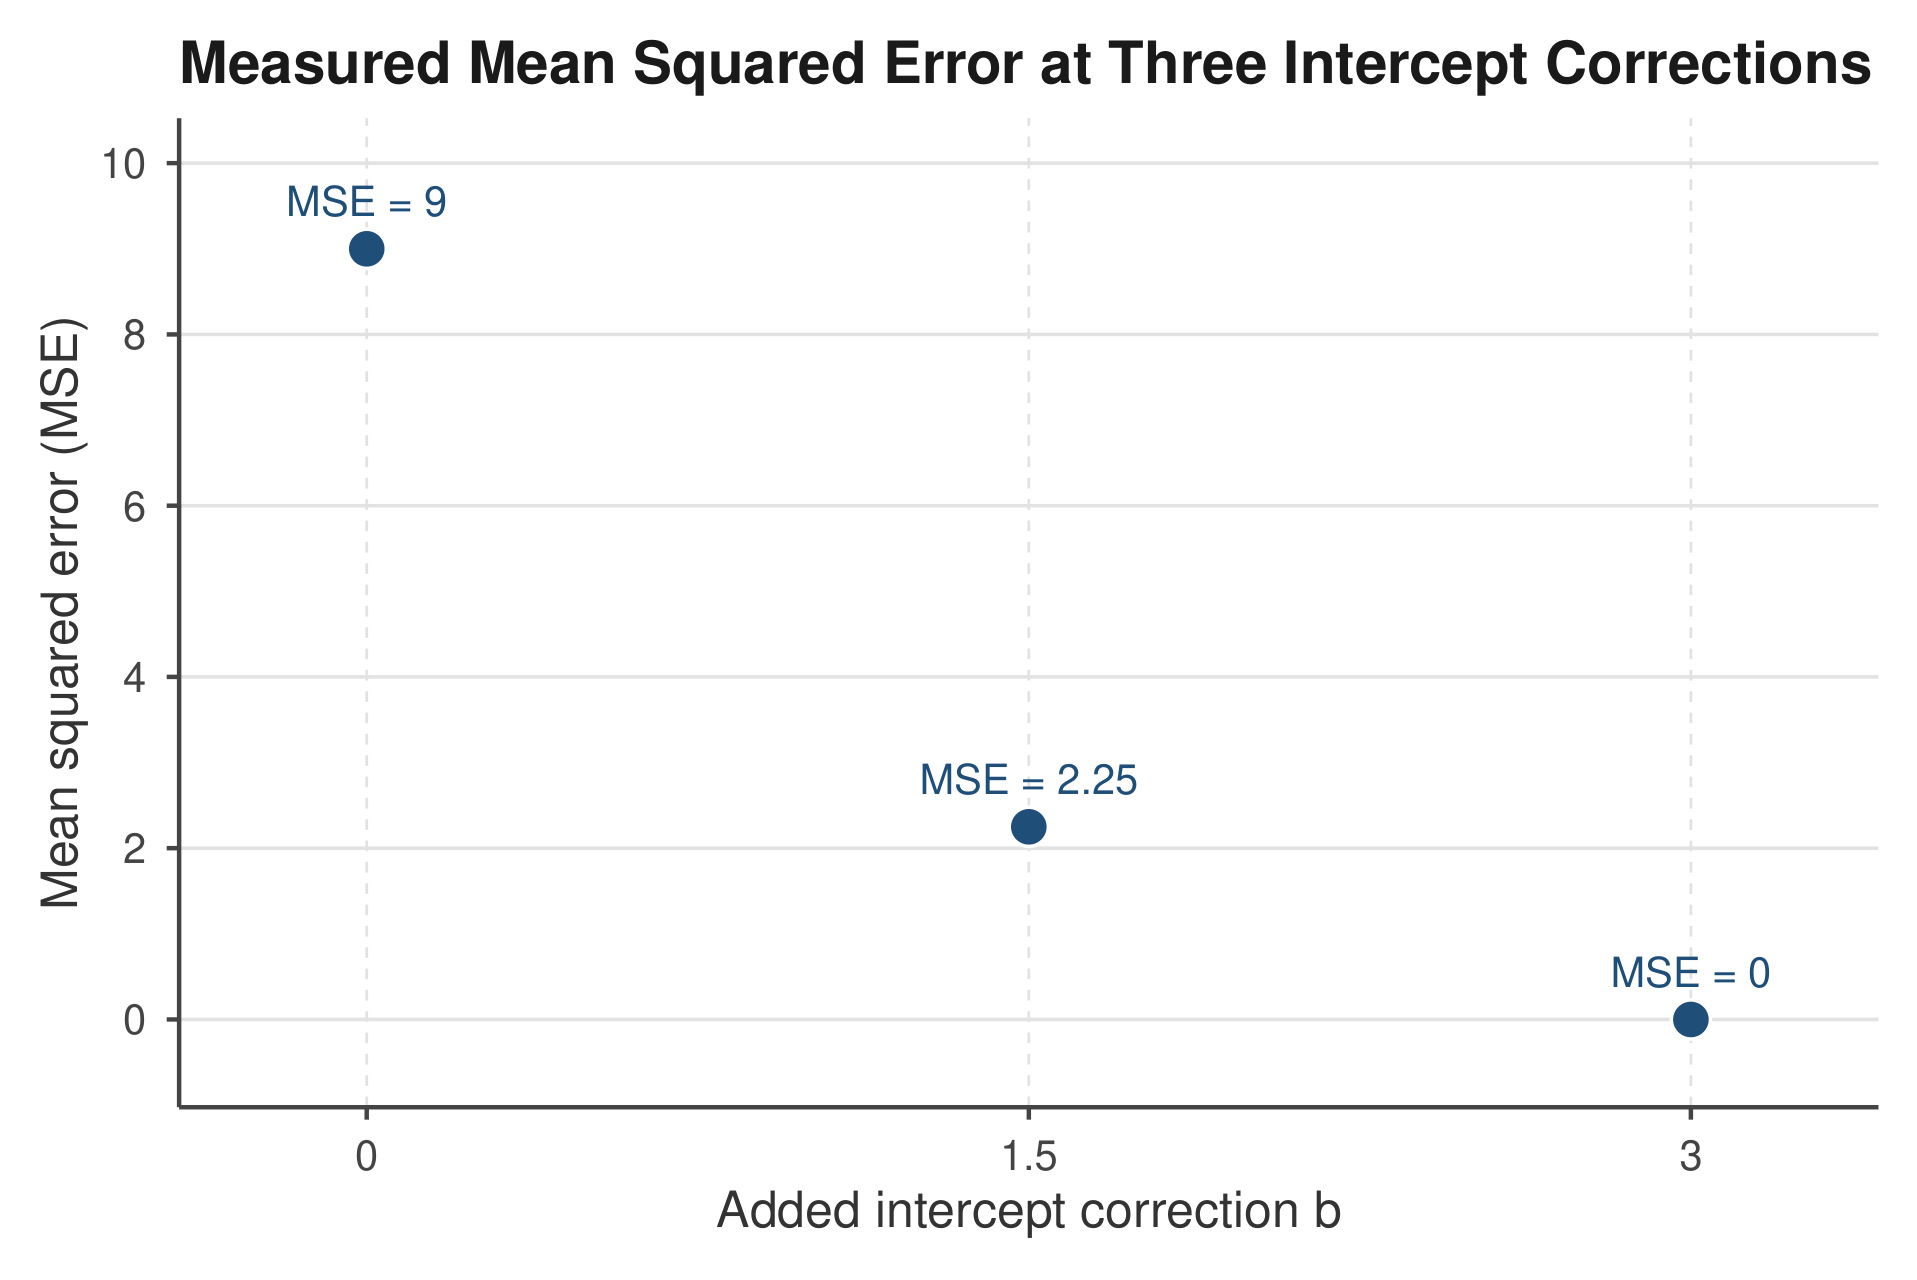
\includegraphics[width=\linewidth]{figures/fig_intercept_error.jpg}
    \caption{The three supplied values
    $(b,\operatorname{MSE})=(0,9),(1.5,2.25),(3,0)$.
    The unchanged graphic's title uses ``Measured'' for values reproduced
    by the deterministic calculation; all three are algebraically determined.
    Each point evaluates the same five observations used for fitting.}
    \label{fig:intercept_error}
\end{figure}

\section{Conclusion}

The five-point calculation connects mean-residual correction to least-squares intercept fitting with a fixed baseline. Its constant residuals explain exact agreement at $b=3$, and its intermediate offset illustrates absolute versus squared error aggregation. The instructional outcome is a traceable account of what is supplied, what is fitted, and what the resulting in-sample errors describe.

\begin{thebibliography}{9}

\bibitem{Anscombe1963ExaminationAnalysis}
Francis John Anscombe and John W. Tukey.
\newblock The Examination and Analysis of Residuals.
\newblock \emph{Technometrics}, 1963.

\bibitem{Gneiting2011MakingEvaluating}
Tilmann Gneiting.
\newblock Making and Evaluating Point Forecasts.
\newblock \emph{Journal of the American Statistical Association}, 2011.

\bibitem{Efron1986HowBiased}
Bradley Efron.
\newblock How Biased is the Apparent Error Rate of a Prediction Rule?
\newblock \emph{Journal of the American Statistical Association}, 1986.

\end{thebibliography}

% PAPER_ORCHESTRA_PROVENANCE_BEGIN
\clearpage
\section*{Figure source provenance}
The files below are the exact sources that produced the embedded figure previews. Paths are relative to this manuscript's source directory. The accompanying \texttt{figure\char95{}provenance.json} records all artifact checksums.\par
\medskip\noindent\textbf{Figure~\ref{fig:intercept_error} (\texttt{fig\char95{}intercept\char95{}error.jpg}).}\par
\noindent R/ggplot2 source: \texttt{figure\char95{}code/\allowbreak{}fig\char95{}intercept\char95{}error/\allowbreak{}source.R}.\par
\noindent Source SHA256: \texttt{2479e40e\allowbreak{}8d39e8e1\allowbreak{}6c29f883\allowbreak{}7e3b8df9\allowbreak{}909f9f65\allowbreak{}8bb35b95\allowbreak{}9fda0b12\allowbreak{}96debbe4}.\par
\noindent Rendering metadata: \texttt{figure\char95{}code/\allowbreak{}fig\char95{}intercept\char95{}error/\allowbreak{}render.json}.\par
\noindent Exact export wrapper: \texttt{figure\char95{}code/\allowbreak{}fig\char95{}intercept\char95{}error/\allowbreak{}worker.R}.\par
\noindent Wrapper SHA256: \texttt{1aedad4b\allowbreak{}1547d4b2\allowbreak{}d394cbb0\allowbreak{}239655d3\allowbreak{}667d453d\allowbreak{}d1fd0eca\allowbreak{}3e77c037\allowbreak{}e6d34892}.\par
\noindent Rendering metadata: \texttt{figure\char95{}code/\allowbreak{}fig\char95{}intercept\char95{}error/\allowbreak{}sessionInfo.txt}.\par
\medskip\noindent\textbf{Figure~\ref{fig:residual_workflow} (\texttt{fig\char95{}residual\char95{}workflow.jpg}).}\par
\noindent LaTeX/TikZ source: \texttt{figure\char95{}code/\allowbreak{}fig\char95{}residual\char95{}workflow/\allowbreak{}source.tex}.\par
\noindent Source SHA256: \texttt{84e305cc\allowbreak{}09efdeb2\allowbreak{}bc2162c3\allowbreak{}9fc60cb1\allowbreak{}d1a3c538\allowbreak{}4254d368\allowbreak{}dee04e8d\allowbreak{}b66664b4}.\par
\noindent Rendering metadata: \texttt{figure\char95{}code/\allowbreak{}fig\char95{}residual\char95{}workflow/\allowbreak{}render.json}.\par
% PAPER_ORCHESTRA_PROVENANCE_END
\end{document}